\section{Spannungsabfall}
Herkömmliche Cat5-Ethernetkabel wurden ursprünglich nicht für die Übertragung großer elektrischer Leistungen entwickelt und besitzen daher Leitungen mit einem sehr geringen Ader-Durchmesser.
Aufgrund dieser Gegebenheit kann es bei weiten Entfernungen oder großen übertragenen Leistungen zu abnormal hohen Spannungsabfällen kommen.
Um die Anlage in dieser Hinsicht zu überprüfen, werden sämtliche Spannungsabfälle und die damit verbundenen Verlustleistungen bei maximaler Belastung durch die Stationen berechnet.
Zur Berechnung der Spannungsabfälle sind folgende Angaben verwendet worden.
\begin{itemize}
	\item Es werden vier Stationen über \ac{poe} versorgt.
	Die Stationen sind nach Abbildung \ref{fig:poe-verdrahtung} miteinander verdrahtet.
	\item Jede Station hat einen maximalen Leistungsverbrauch von 12 W.
	\item Das Ethernetkabel zwischen den Stationen hat jeweils eine Länge von 10 m.
	\item Der Querschnitt einer Ader des Ethernet-Kabels beträgt 0.128 mm\textsuperscript{2} \cite[vgl.][]{lapp-cat5-datasheet}.
	\item Am \ac{pse} wird eine Spannung von 30 V in das Netz eingespeist.
\end{itemize}
\begin{figure}[htbp!]
	\centering
	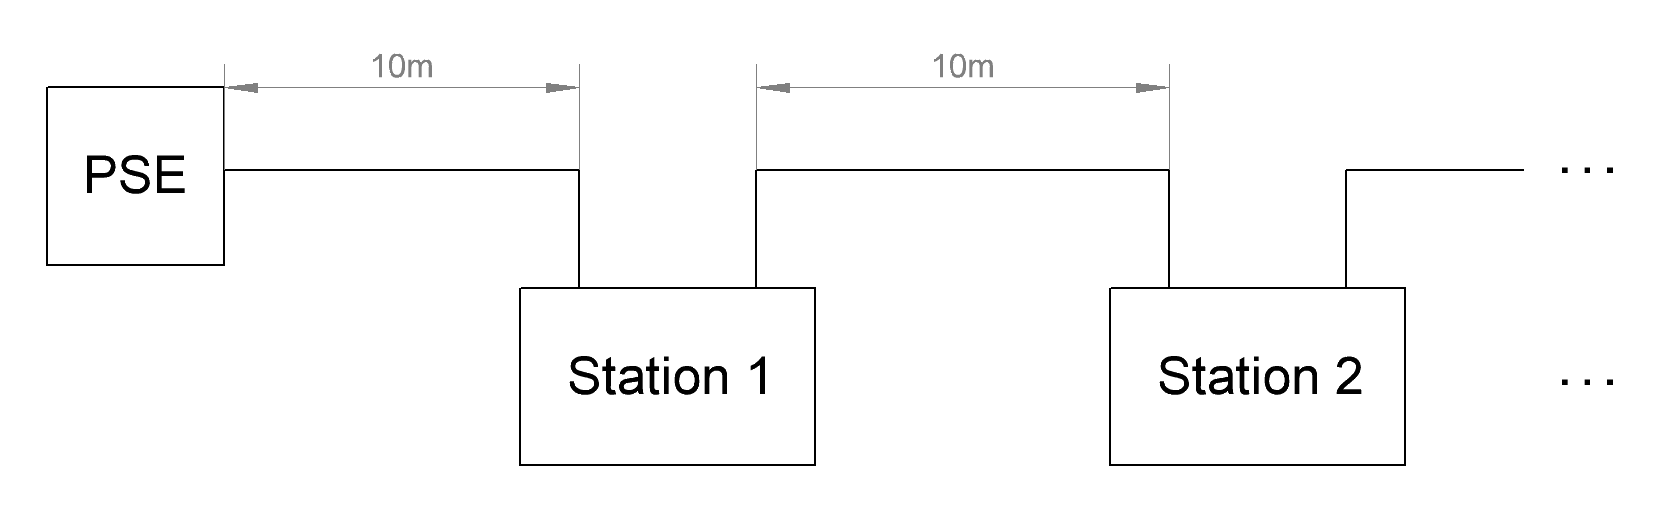
\includegraphics[width=.9\linewidth]{images/berechnung/poe_verdrahtung.png}
	\caption{Verdrahtungsschema}
	\label{fig:poe-verdrahtung}
\end{figure}
Der Leitungswiderstand eines Adernpaares des Ethernetkabels beträgt nach der allgemeinen Drahtwiderstandsformel $R_{Ltg}=\frac{l}{\gamma\cdot A}=0.686\Omega$.
Bei den \ac{poe}-Typen 1 und 2 wird je ein Adernpaar für die Zu- und Rückleitung verwendet.
Bei den \ac{poe}-Typen 3 und 4 werden je zwei Adernpaare parallel geschaltet.\par

Daraus ergeben sich die in den Abbildungen \ref{fig:ers-type12} und \ref{fig:ers-type34} dargestellten Ersatzschaltungen.
Die Stationen (Verbraucher) sind als Widerstand gezeichnet, wobei sie sich nicht wie ein solcher verhalten.
\begin{figure}[htbp!]
	\centering
	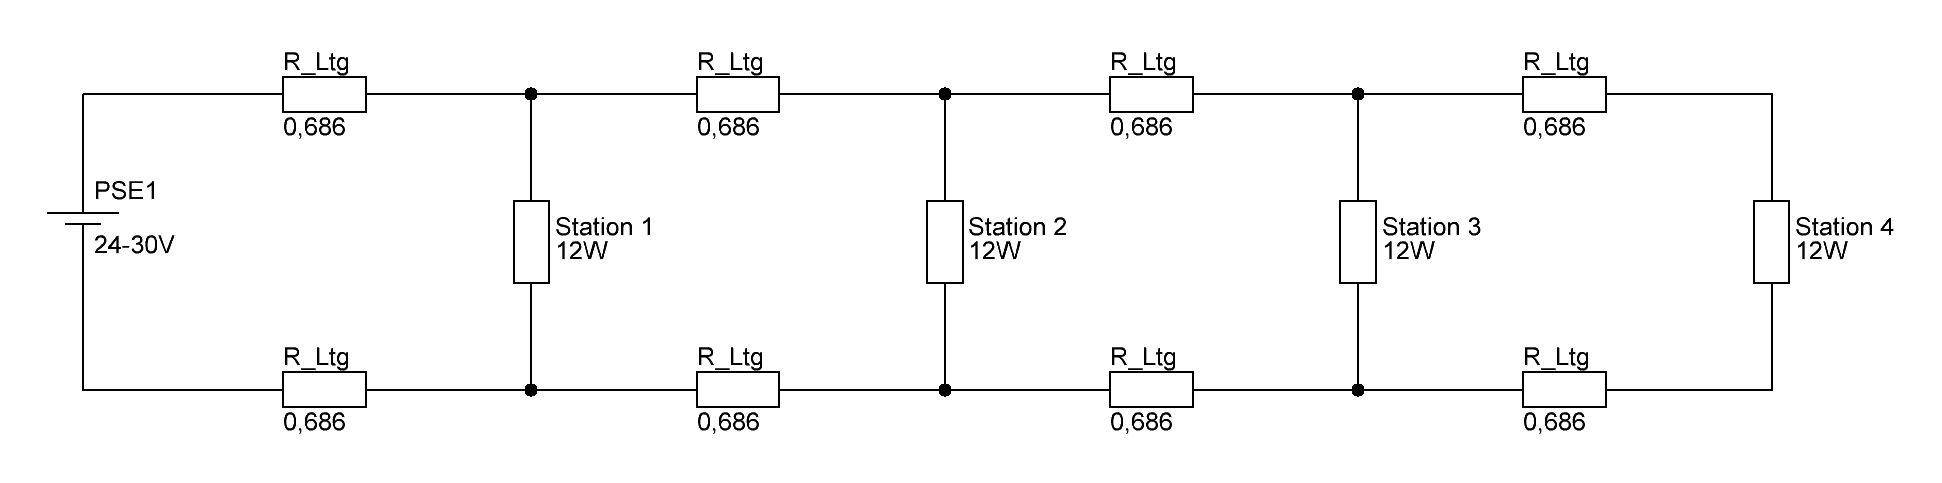
\includegraphics[width=\linewidth]{images/berechnung/poe2pair.png}
	\caption{Ersatzschaltung  \ac{poe} Type 1 und 2}
	\label{fig:ers-type12}
\end{figure}
\begin{figure}[htbp!]
	\centering
	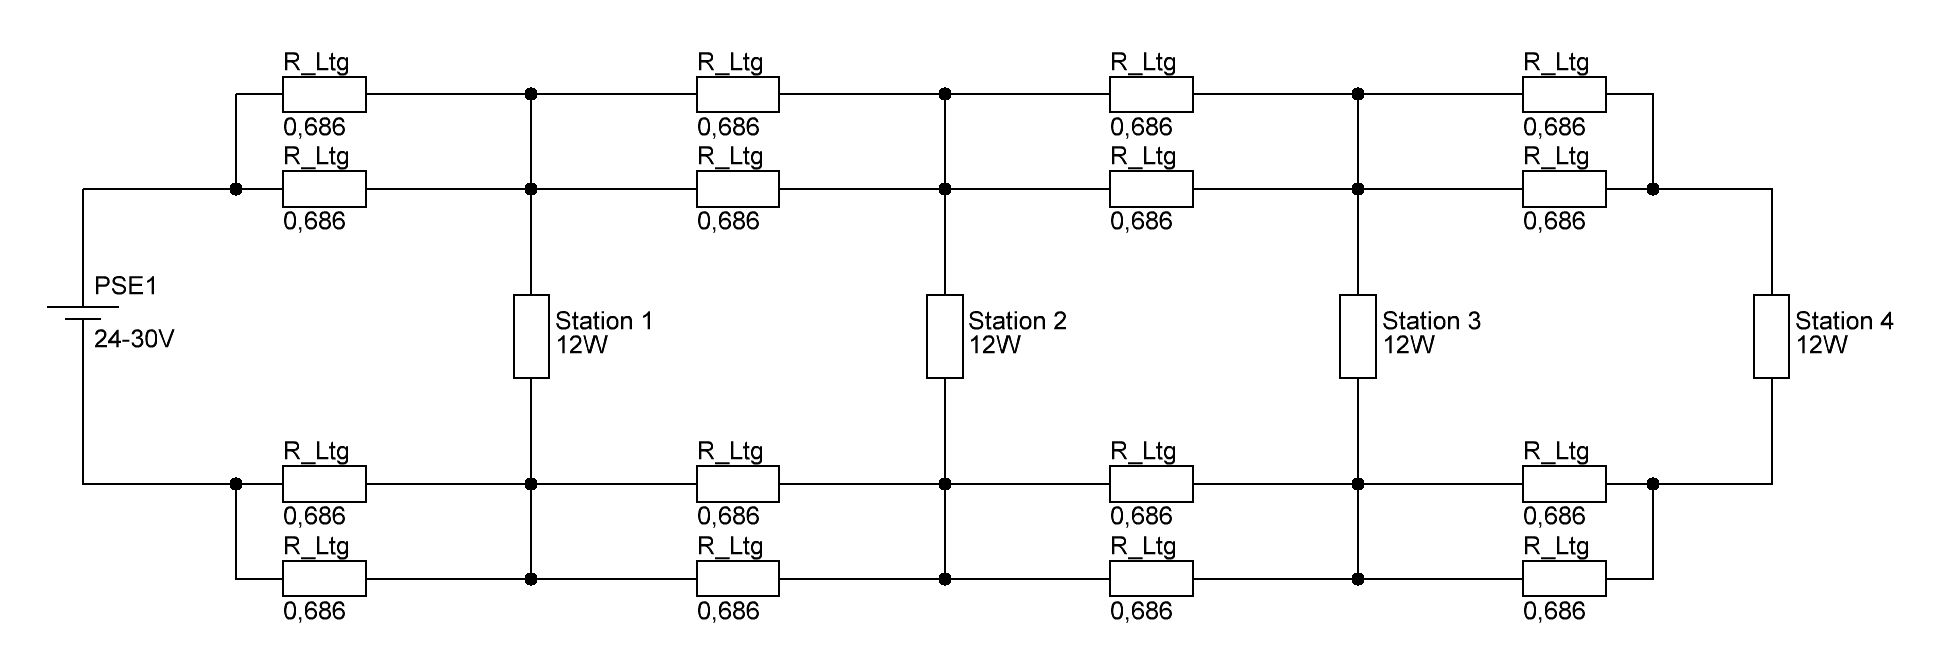
\includegraphics[width=\linewidth]{images/berechnung/poe4pair_neu.jpg}
	\caption{Ersatzschaltung  \ac{poe} Type 3 und 4}
	\label{fig:ers-type34}
\end{figure}

Anhand der in den Abbildungen \ref{fig:ers-type12} dargestellten Ersatzschaltung ergibt sich ein Gleichungssystem in 8 Variablen.
Für die in Abbildung \ref{fig:ers-type34} dargestelle Ersatzschaltung halbiert sich der Leitungswiderstand, wodurch der Faktor 2 vor diesem in den Gleichungen verschwindet.
Die Quellenspannung ist mit U\textsubscript{0} bezeichnet, der Strom und die Spannung der Station n mit I\textsubscript{n} bzw. U\textsubscript{n}.
\begin{align}
	U_1 &= U_0-2\cdot R_{Ltg}\cdot (I_1+I_2+I_3+I_4)\\
	U_2 &= U_1-2\cdot R_{Ltg}\cdot (I_2+I_3+I_4)\\
	U_3 &= U_2-2\cdot R_{Ltg}\cdot (I_3+I_4)\\
	U_4 &= U_3-2\cdot R_{Ltg}\cdot I_4\\
	12W &= U_1\cdot I_1\\
	12W &= U_2\cdot I_2\\
	12W &= U_3\cdot I_3\\
	12W &= U_4\cdot I_4
\end{align}

Dieses Gleichungssystem von Hand zu lösen, würde viel Zeit in Anspruch nehmen.
Daher wurde für die Lösung auf das Computerprogramm wxMaxima zurückgegriffen.
Die Eingabe der Gleichungen erfolgt in Textform (siehe Abbildung \ref{fig:maxima-input})\par

wxMaxima ist eine dokumentenbasierte Schnittstelle für das Computeralgebrasystem Maxima. wxMaxima bietet Menüs und Dialoge für viele gängige Maxima-Befehle, Autovervollständigung, Inline-Plots und einfache Animationen. wxMaxima wird unter der \ac{gpl} vertrieben. \cite[aus dem Englischen übersetzt]{wxmaxima}\par

\begin{figure}[htbp!]
	\centering
	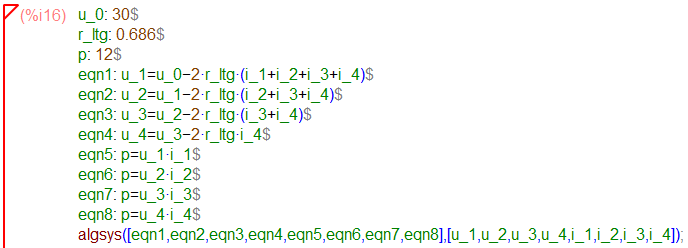
\includegraphics[width=.9\linewidth]{images/berechnung/max_2pair_30V.png}
	\caption{Eingabe wxMaxima Type 1 \& 2}
	\label{fig:maxima-input}
\end{figure}

Die Lösungen für das Gleichungssystem werden vom Programm in Textform zurückgegeben.
Das Programm findet neben der relevanten Lösung noch einige komplexe Lösungen für das Gleichungssystem.
Diese werden hier aus Platzgründen und geringer Relevanz weggelassen.
\begin{table}[htbp!]
	\centering
	\begin{tabular}{r|ccc|ccc}
		\toprule
		&\multicolumn{3}{c|}{Type 1 \& 2}&\multicolumn{3}{c}{Type 3 \& 4}\\\cmidrule{2-7}
		&U&\tdelta U&I&U&\tdelta U&I\\
		\midrule
		Quelle&30.00 V&&1931 mA&30.00 V&&1729 mA\\
		\midrule
		Station 1&27.35 V& 8.83\%&438 mA&28.81 V& 3.97\%&416 mA\\
		Station 2&25.30 V&15.67\%&474 mA&27.91 V& 6.97\%&430 mA\\
		Station 3&23.90 V&20.33\%&502 mA&27.31 V& 8.97\%&439 mA\\
		Station 4&23.19 V&22.70\%&517 mA&27.00 V&10.00\%&444 mA\\
		\bottomrule
	\end{tabular}
	\caption{Berechnung Ergebnisse}
\end{table}
Bei einer Quellenspannung von 30 V und einem Gesamtstrom von 1.931 A (Type 1 \& 2) bzw. 1.729 A (Type 3 \& 4) ergibt sich eine Gesamtleistung von 57.93 bzw. 51.87 W.
Bei Type 3 \& 4 ist die Belastung der Quelle um 10 \% niedriger als bei Type 1 \& 2.

Man sieht: Der Spannungsabfall ist wie erwartet bei Type 3 und 4 weniger als halb so groß als bei Type 1 und 2.
Dadurch ist auch die gesamte Verlustleistung der Leitungen geringer, was eine niedrigere Belastung der Quelle bedeutet.

Aus der obigen Rechnung ergibt sich, dass für die gegebene Anlage eine Versorgung nach Type 3 bzw. 4 empfehlenswert ist.